\documentclass[../Bachelorarbeit.tex]{subfiles}

\begin{document}
\label{sec:EFT}
With the Standard Model (\acrshort{sm}) physicist try to describe the elementary particles and interactions. It is successful in describing most processes in physics.
But the \acrshort{sm} is still incomplete. It can't describe phenomenons like gravity, neutrino masses, matter-antimatter asymmetry etc. This is where effective field theory (\acrshort{eft}) comes in.
Here one looks at the \acrshort{sm} as a low energy approximation of an underlying ultraviolet(\acrshort{uv}) theory (figure~\ref{fig:EFT_sketch}). An in depth introduction into \acrshort{eft} is shown in \cite{Pich.1998} and \cite{Brivio.2019}.

\begin{figure}[h]
    \centering
    \includegraphics[width=0.5\textwidth]{images/EFT_Model.png}
    \caption{Sketch of the Basic \acrshort{eft} concept with the low energy observer having energy E and cutoff at $\Lambda$. The \acrshort{sm} and \acrshort{bsm} theory(here GM H5 Model \cite{Kundu.28.11.2021}) are combined in the \acrshort{eft}. \cite{Brivio.2017}}
    \label{fig:EFT_sketch}
\end{figure}
%-------------------------------------------------------------------------------------Fermi Theory-------------------------------------------------------------------------------------------------------
\subsection{Fermi Theory on the example Tau Decay}
\label{sec:Fermi}
In 1933 Enrico Fermi proposed the Fermi theory in order to describe the $\beta$-decay. His theory was able to describe the
weak coupling quite well without the former knowledge about the $W^{\pm}$-Boson which was only later theorized in 1968 by Steven Weinberg, Sheldon Glashow and Abdus Salam.
The $W^{\pm}$-Boson was finally discovered in 1983. 50 years after Fermi's first successful description of an interaction involving the $W^{\pm}$-Boson.
Today one would call the Fermi theory the low-energy \acrshort{eft} of the $W^{\pm}$-Boson.
Let's try now to create a different Fermi theory but instead of describing the $\beta$ decay\cite{Thomson.2013}, this theory will look at the $\tau$-decay specifically the decay mode $\tau \rightarrow \nu_{\tau}e^{-}\nu_{e}$.
Even though this is technically cheating since Fermi didn't have modern knowledge about the tensor structure of the weak interaction in Quantum Field Theory or the knowledge about Feynman diagrams.
One can start by drawing the Feynman diagram and writing down the Lorenz invariant matrix element.
\begin{figure}[h]
    \centering
    \includegraphics[width=0.5\textwidth]{images/Feynamn_tau_decay.PNG}
\end{figure}

\begin{equation}
    -i\mathcal{M}_{fi}= \left[ \frac{g_{W}}{\sqrt{2}} \overline{u}(k_{\nu_{\tau}})\frac{1}{2}\gamma^{\mu}(1-\gamma^{5})u(k_{\tau}) \right] \frac{g_{\mu\sigma}-\frac{k_{\nu}k_{\sigma}}{m_{W}^{2}}}{k^{2}-m_{W}^{2}} \left[ \frac{g_{W}}{\sqrt{2}} \overline{u}(k_{e})\frac{1}{2}\gamma^{\sigma}(1-\gamma^{5})v(k_{\overline{\nu_{e}}}) \right]
\end{equation}

In most low energy decay processes the momentum of the intermediate $W^{-}$-Boson is small compared to its mass. Therefore, one can approximate the
propagator (\ref{eq:Fermi_propergator}) in orders of the momentum $k$. But the matrix element in here written in orders
of mass since these are more interesting for this thesis. In the Feynman diagram this can be expressed by collapsing the propagator into a single vertex.

\begin{figure}[h]
    \centering
    \includegraphics[width=0.5\textwidth]{images/propagator_collaps.PNG}
\end{figure}
\begin{equation}
    \frac{-ig_{\mu\sigma}-\frac{k_{\nu}k_{\sigma}}{m_{W}^{2}}}{k^{2}-m_{W}^{2}} \xrightarrow{\abs{k}^{2} \ll m_{W}^{2}} \frac{ig_{\mu\sigma}}{m_{W}^{2}} \left( 1 + \frac{k^{2}}{m_{w}^{2}}+\frac{k^{4}}{m_{W}^{6}}+\mathcal{O}(k^6) \right)
    \label{eq:Fermi_propergator}
\end{equation}

\begin{equation}
    \Rightarrow i\mathcal{M}_{fi}=\frac{g_{W}^{2}}{8 m_{W}^{2}} \left[ \overline{u}(k_{\nu_{\tau}})\gamma^{\mu}(1-\gamma^{5})u(k_{\tau}) \right] g_{\mu\sigma} \left[ \overline{u}(k_{e})\gamma^{\sigma}(1-\gamma^{5})v(k_{\overline{\nu_{e}}}) \right] + \mathcal{O}(m_{W}^{4})
    \label{eq:Fermi_colapse}
\end{equation}

One can now compare the result with the result Fermi would have gotten if he knew about the parity violation discovered by Wu in 1957.

\begin{equation}
    i\mathcal{M}_{fi} = \frac{G_{F}}{\sqrt{2}} \left[ \overline{u}(k_{\nu_{\tau}})\gamma^{\mu}(1-\gamma^{5})u(k_{\tau}) \right] g_{\mu\sigma} \left[ \overline{u}(k_{e})\gamma^{\sigma}(1-\gamma^{5})v(k_{\overline{\nu_{e}}}) \right]
    \label{eq:Fermi_the_slim_Fermi}
\end{equation}
With $G_{F} \approx 4.5437957\times 10^{14} J^{-2}$ being the Fermi constant which is typically measured in the muon decay. The $1/\sqrt{2}$ is added in order to not change the numerical value of $G_{F}$ while considering the parity violation.
From equation \ref{eq:Fermi_colapse} and \ref{eq:Fermi_the_slim_Fermi} on gets the following result.
\begin{equation}
    \frac{G_{F}}{\sqrt{2}} = \frac{g_{W}^{2}}{8 m_{W}^{2}}
\end{equation}
Defining the expansion scale $\Lambda=m_{W}$ and the Wilson coefficient $c= \frac{g_{W}^{2}}{8}$ one can see that the matrix element has dimension 2.
With this one can also write down a new effective Lagrangian without the $W^{\pm }$-Boson. But the \acrshort{eft} described has to contain the tau, electron, their respective neutrino fields
as well as the interaction Lagrangian.
\begin{equation}
    \mathcal{L}_{EFT} = \frac{c}{\Lambda^{2}} \left( \overline{\nu}_{\tau} \overline{\gamma}_{\rho} \tau \right) \left(\bar{e} \overline{\gamma}_{\rho} \nu_{e} \right) + \mathcal{O}(\frac{1}{\Lambda^{4}})
\end{equation}
This Fermi theory is only valid for low energies since the scattering amplitude from the \acrshort{sm} and the \acrshort{eft} would
start to diverge once the energy gets close to the mass of the $W^{\pm}$-Boson.
The $m_{W}$ defines the validity scale of the \acrshort{eft} in this case the Fermi theory. For energies higher than $m_{W}$ the
Fermi theory is no longer valid. One can increase the validity scale by including therms of higher dimension in $\Lambda$.
In this example the Matrix element was derived from the \acrshort{sm} and then compared the result with the result from Fermi in
order to determine $\frac{c}{\Lambda}$. This requires knowledge about the \acrshort{uv} theory which is not accessible in low-Energy
measurements. As a result one has to make assumptions about the \acrshort{uv} theory in order to construct the right \acrshort{eft}. This is called \acrshort{eft} Matching. The concept is shown in figure \ref{fig:matching}.

%We can now use the Fermi Theory for low mass Measurements ($m_{l} \ll m_{W}$) like the tau decay to calculate the Decay width
%by integrating the matrix element squared over the phase space of each finale state particle. I will only quote the result her, sice the acctuale calculations proves to be quite long but can be looked at here \cite{Quelle für Die myon decay rechnung}.
%
%\begin{equation}
%    \Gamma(\tau \rightarrow \nu_{\tau} e^{-} \overline{\nu_{e}}) = \frac{G_{F}^{2} m_{\tau}^{5}}{192 \pi^{3}} f \left(\frac{m_{e}^{2}}{m_{\tau}^{2}} \right) \textnormal{ with } f(x)=1-8x-8x^{3}-x^{4}-12 x^{2} ln(x)
%\end{equation}
\begin{figure}
    \centering
    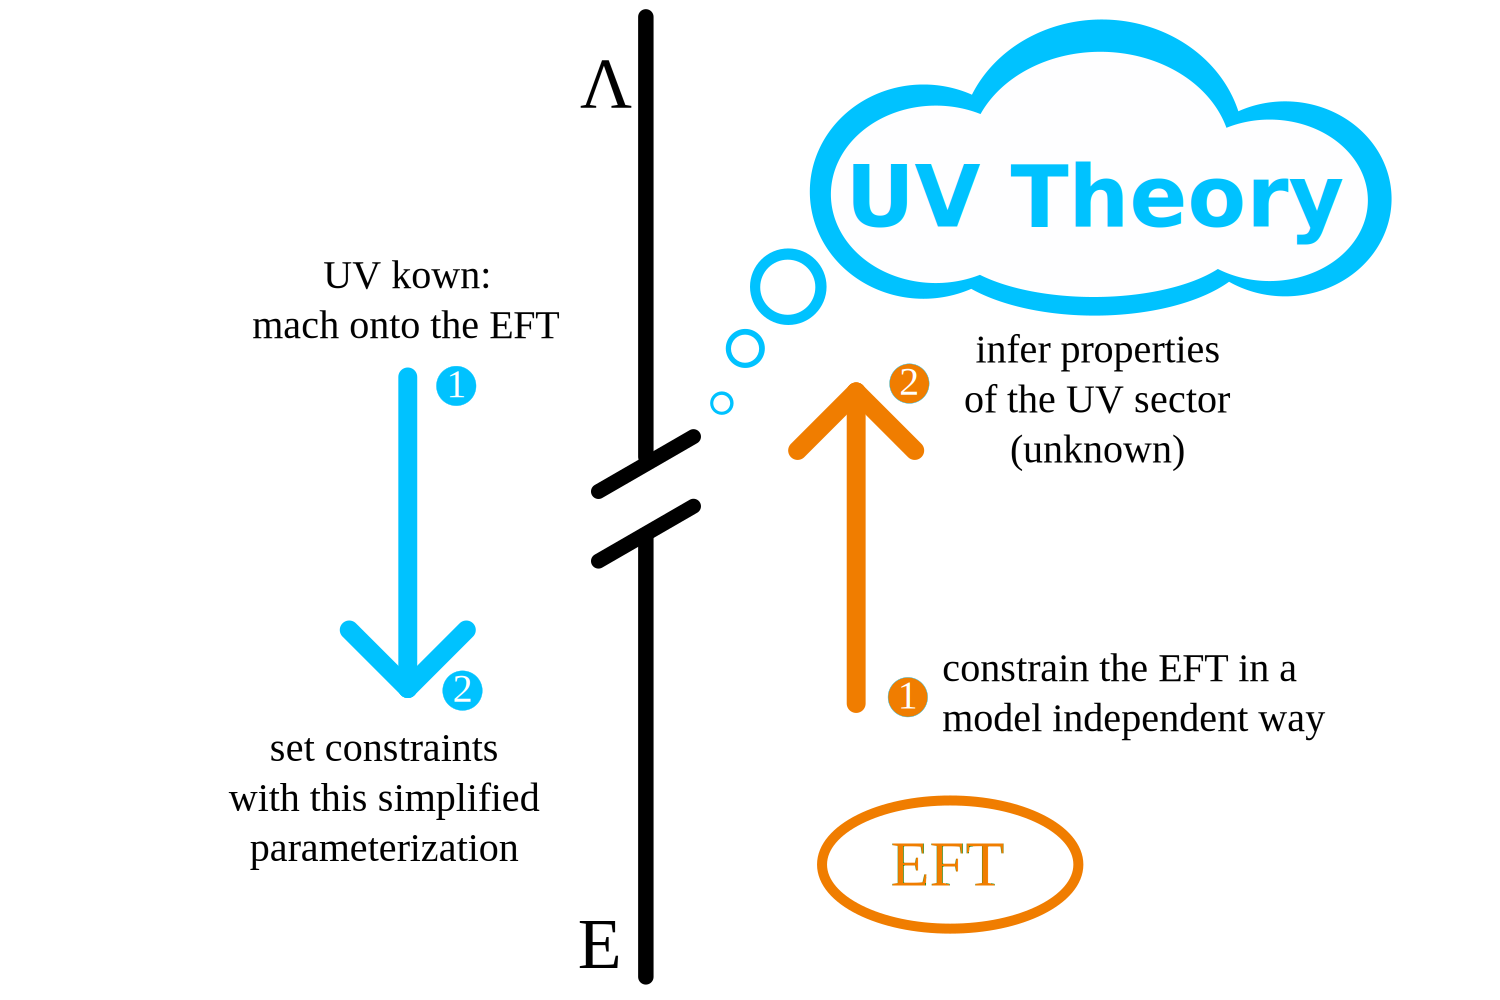
\includegraphics[width=0.5\textwidth]{images/EFT_matching.png}
    \caption{Schematic representation for the matching of an \acrshort{eft} to the \acrshort{uv} theory using top-down and bottom-up matching method. \cite{Brivio.}}
    \label{fig:matching}
\end{figure}

\subsection{Standard Model Effective Field Theory (\acrshort{smeft})}
As the Name suggests The \acrfull{smeft}\cite{Pich.1998} aims to extend the \acrshort{sm}.
Except the g-Factor of the myon the \acrshort{sm} has been robust without meaningful deviations from experimental measurements.
%With that in mind it is reasonable to assume that new Particles are heavier than Particles within the weak scale. 
%This allows the \acrshort{smeft} a Model-indepentent way to describe Beyond the Standard Model effects.
For this reason using a theory that keeps the $SU(3) \times SU(2) \times U(1)$ symmetry with the Higgs field breaking gauge symmetry is desirable.
One can construct the Lagrangian from the gauge invariance of \acrshort{sm} fields and allow arbitrarily large mass dimensions.
With that any \acrshort{smeft} Lagrangian can be written as:

\begin{equation}
    \mathcal{L}_{SMEFT} = \mathcal{L}_{SM} + \frac{1}{\Lambda} \mathcal{L}_{5} + \frac{1}{\Lambda^2} \mathcal{L}_{6} + \frac{1}{\Lambda^3} \mathcal{L}_{7} + \frac{1}{\Lambda^4} \mathcal{L}_{8} + ... \textnormal{ with } \mathcal{L}_{i} = \sum_{i} c_{i}^{D} \mathcal{O}_{i}^{D}
    \label{eq:L_SMEFT}
\end{equation}

The operators $\mathcal{O}_{i}$ are constructed from the gauge invariance of the \acrshort{sm} fields while the Wilson coefficients $c_{i}$ contain the information on heavy degrees of freedom.
Normally the heavy degrees of freedom are integrated out to have a renormalizable theory but are needed to describe high energy particles.
The Wilson coefficients are constructed from the operator product expansion in \ref{eq:L_SMEFT} as shown in the Fermi theory(\ref{sec:Fermi}).
For a characteristic heavy scale $\Lambda$ the operators are ordered by there dimension $d_{i}$ fixing the dimension of their respective coefficients.

\begin{equation}
    [\mathcal{O}_i] = d_{i} \longrightarrow c_{i} \sim \frac{1}{\Lambda^{d_{i}-4}}
\end{equation}

The leading order $D = 4$ (marginal operator) term in \ref{eq:L_SMEFT} is the \acrshort{sm} Lagrangian while deviations of the \acrshort{sm} are described by operators with a dimension $D>4$ also called irrelevant operators since they are suppressed by the scale $E/ \Lambda$.
Even though they are called irrelevant they often contain important information for processes with high energy. In a Fermi theory these contain information about processes with leading order flavour-change.
Relevant operators $D<4$ become relevant for energies close to the validity scale and only \acrshort{eft}'s with relevant and marginal operators are normalizable making the predictions valid up to $E/\Lambda$.
\\\\
Using knowledge about \acrshort{sm} fields and known symmetries one can construct an operator basis. All allowed invariant structures are found using the \acrshort{sm} fields and their symmetries at a dimension D.
Removing all terms from the S-matrix that would result in the same physics provides the basis. The General choice of basis in the search for new physics is the Warsaw basis \cite{Brivio.}, other basis can be chosen as physics should be basis independent.
In vector boson scattering (\acrshort{vbs}) processes the Eboli basis\cite{EleniVryonidou.15.02.2019} is commonly used because the operators can be categorized in longitudinal operators only containing covariant derivatives $D^{\mu}$ and a Higgs doublet fields $\Phi$,
transverse operators only containing field strength tensors $\widehat{W}_{\mu\nu}$ and mixed operators containing combinations.
Most of the operators can be discarded since they don't contribute to $W^{\pm}Z$ processes leaving only six dimension-8 operators.
\\
\begin{table}[h]
    \centering
    \begin{tabular}{ l c }
        Longitudinal: & $\mathcal{O}_{S,1} = [(D_{\mu}\Phi)^{\dagger} D_{\mu}\Phi] \times [(D^{\nu}\Phi)^{\dagger} D^{\nu}\Phi]$                         \\
                      &                                                                                                                                  \\
        Mixed:        & $\mathcal{O}_{M,0} = Tr[\widehat{W}_{\mu\nu}\widehat{W}^{\mu\nu}] \times [(D_{\beta}\Phi)^{\dagger} D^{\beta}\Phi]$              \\
                      & $\mathcal{O}_{M,1} = Tr[\widehat{W}_{\mu\nu}\widehat{W}^{\mu\beta}] \times [(D_{\beta}\Phi)^{\dagger} D^{\mu}\Phi]$              \\
                      &                                                                                                                                  \\
        Transverse:   & $\mathcal{O}_{T,0} = Tr[\widehat{W}_{\mu\nu}\widehat{W}^{\mu\nu}] \times Tr[\widehat{W}_{\alpha\beta}\widehat{W}^{\alpha\beta}]$ \\
                      & $\mathcal{O}_{T,1} = Tr[\widehat{W}_{\alpha\nu}\widehat{W}^{\mu\beta}] \times Tr[\widehat{W}_{\mu\beta}\widehat{W}^{\alpha\nu}]$ \\
                      & $\mathcal{O}_{T,2} = Tr[\widehat{W}_{\alpha\mu}\widehat{W}^{\mu\beta}] \times Tr[\widehat{W}_{\beta\nu}\widehat{W}^{\nu\alpha}]$ \\
    \end{tabular}
\end{table}
\subsection{EFT validity and unitarity violation}
The time evolution of states in quantum mechanics is mathematically described by unitary operators. Time evolution without unitary operators is proposed in new approaches to quantum mechanics like Carl M. Benders talk in 2020 at the TU-Dresden
proposing a quantum theory including non Hermitian Hamiltonian \cite{Prof.Dr.CarlBender.2020}. Unitarity was a decisive concept for the inclusion of the Higgs field in the \acrshort{sm} as it restored unitarity at tree level.
\acrshort{eft} isn't a complete theory by extending the \acrshort{sm}, the triple gauge coupling (\acrshort{tgc}) and quadratic gauge coupling (\acrshort{qgc}) processes are modified leading to unitarity violation. The expected behaviors of a unitary \acrshort{eft} is dim-6 interference > dim-6 quadratic $\sim$ dim-8 interference > dim-8 quadratic.
This however is not the case as dim-8 operators cause the scattering amplitude to grow asymptotically $\sim \Lambda^{2}$. This eventually leads to unitarity violation \ref{fig:dim8_quad_int_comparission}.
\begin{figure}[h]
    \centering
    \begin{subfigure}{0.4\textwidth}
        \centering
        \includegraphics[width=\textwidth]{Plots/int_quad_comparision/all_VV_MWZ_vbs.pdf}
        \caption{}
    \end{subfigure}
    \begin{subfigure}{0.4\textwidth}
        \centering
        \includegraphics[width=\textwidth]{Plots/int_quad_comparision/all_VV_MTWZ.pdf}
        \caption{}
    \end{subfigure}
    \caption{Comparission of inteferenz term and quadratic term for the S1 parameters created with value S1=128. The quadratic therm is bigger for higher energies since no unitarisation is used. \textbf{a)}$M(WZ)$,\textbf{b)}$M_{T}(WZ)$}
    \label{fig:dim8_quad_int_comparission}
\end{figure}
\newpage
One can now apply a cutoff at the validity scale $M=\Lambda$ but in practice the value of $\Lambda$ is unknown and can only be gained by analysing data. This means that \acrshort{eft} predictions are only valid for an operator dependent unitarity limit.
It should be noted that unitarity can be restored by using unitarisation. In ATLAS research the relatively simple K-matrix method is commonen tool for unitarisation as shown in \cite{Kilian.2015}. This however does not restore \acrshort{eft} validity and
makes connecting \acrshort{eft} results to \acrshort{uv} theories harder. In conclusion the search for beyond the standard model(\acrshort{bsm}) effects using \acrshort{eft} is only possible in an energy range as light states are not detectable and high Energy states are removed by the unitarity limit \ref{fig:EFT_validity}.
\begin{figure}[h]
    \centering
    \begin{subfigure}{0.45\textwidth}
        \centering
        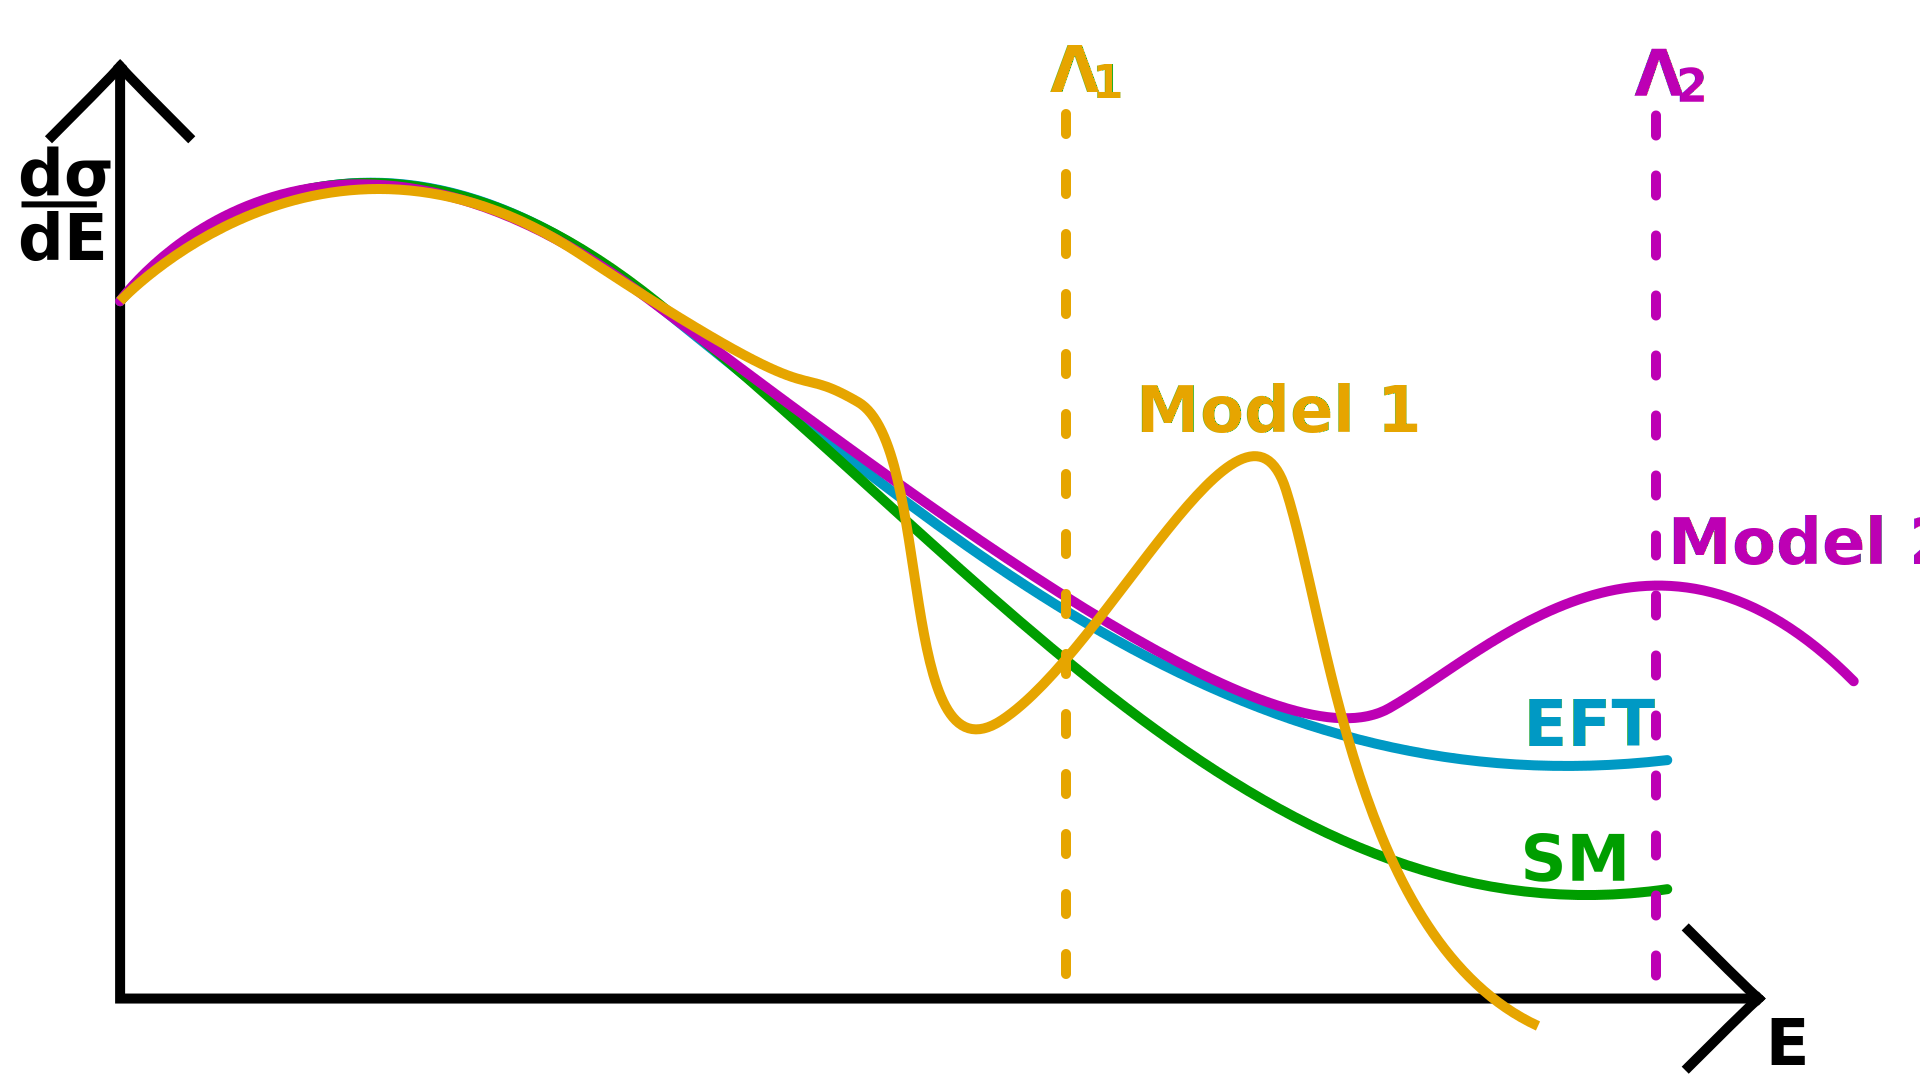
\includegraphics[width=\textwidth]{images/EFT_validity.png}
        \caption{}
    \end{subfigure}
    \begin{subfigure}{0.45\textwidth}
        \centering
        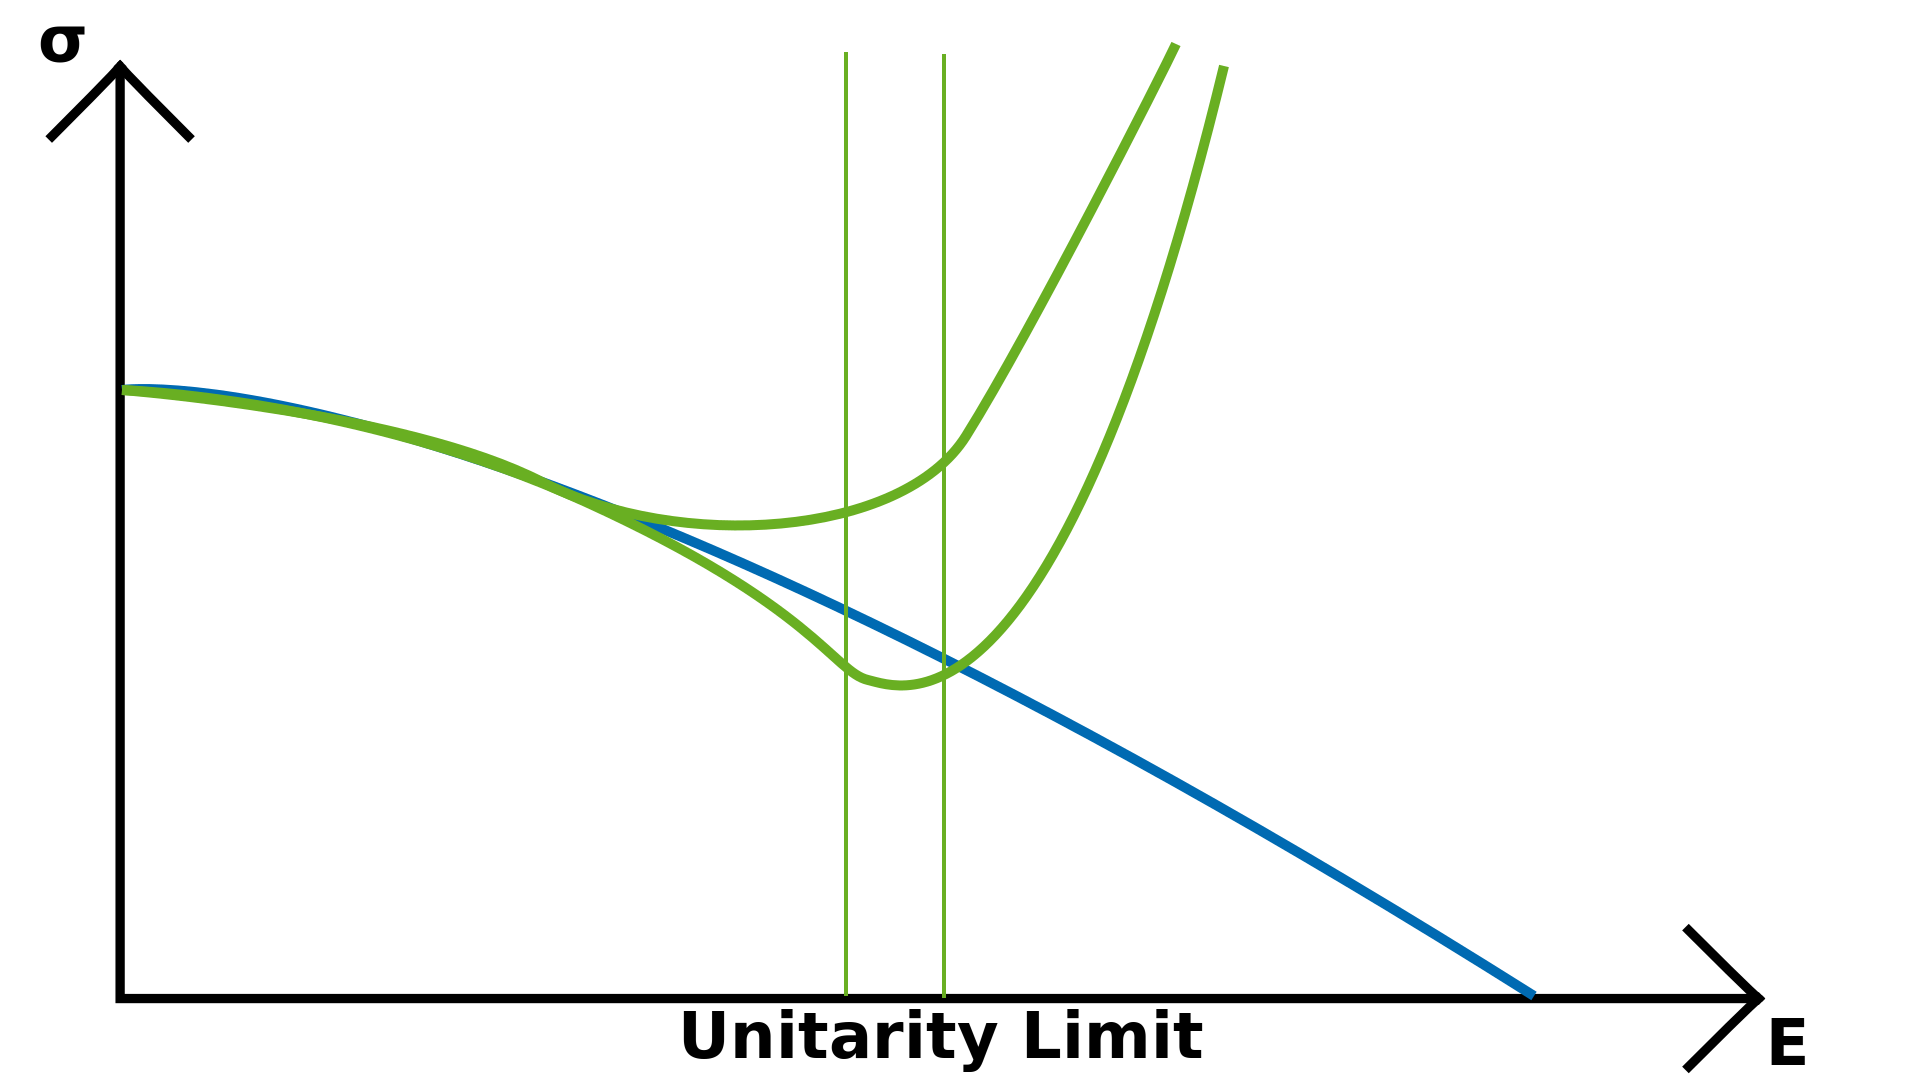
\includegraphics[width=\textwidth]{images/EFT_cross_section.png}
        \caption{}
    \end{subfigure}
    \caption{\textbf{a)} Not all models can be fitted using \acrshort{eft} only ones with energy scale higher than the \acrshort{sm} \cite{Brivio.2017}\textbf{b)} Schematic of unitarity limits the energy range changes depending on the cutoff \cite{MichaSzleper.} }
    \label{fig:EFT_validity}
\end{figure}
\end{document}
